\begin{XeClass}{FileUtil}
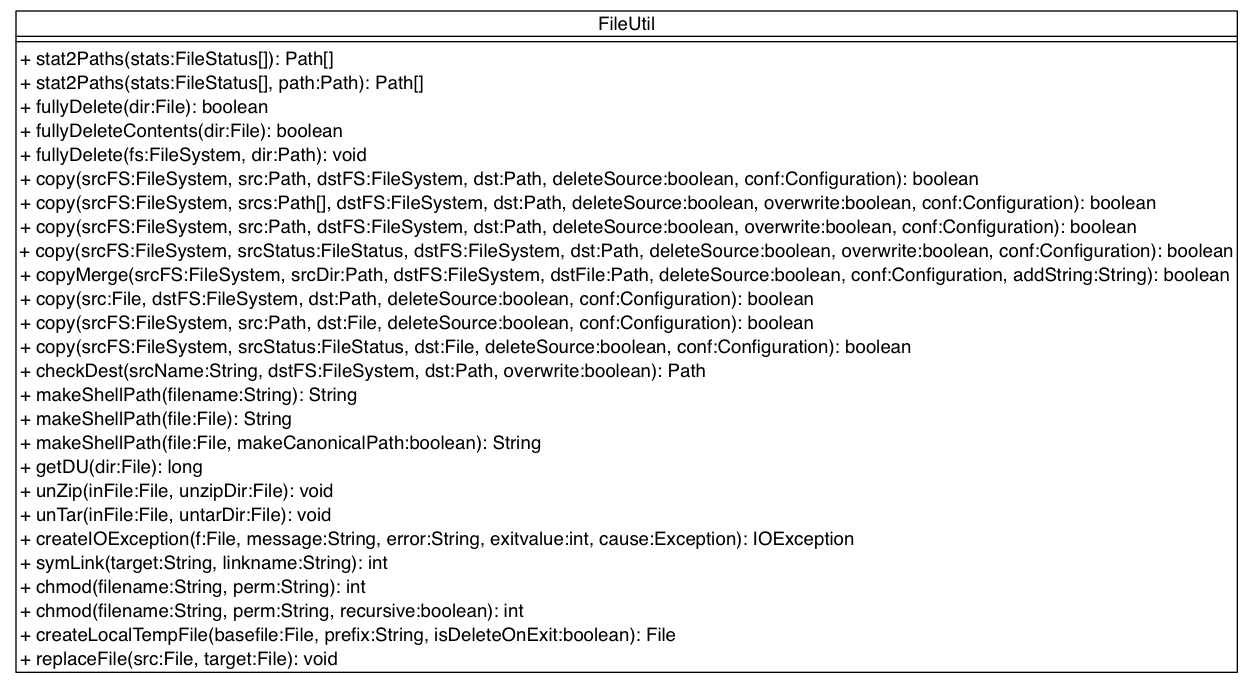
\includegraphics[width=10cm]{cdig/FileUtil.png}
     
 该类通过静态方法提供了大量的文件处理函数

    \begin{XeMethod}{\XePublic}{Path[]}{stat2Paths}
         
 将一个FileStatus数组转化为Path数组,通过调用每个FileStatus
 的getPath()方法实现

    \end{XeMethod}

    \begin{XeMethod}{\XePublic}{Path[]}{stat2Paths}
         
 将一个FileStatus数组转化为Path数组,如果stats为null,则返回path

    \end{XeMethod}

    \begin{XeMethod}{\XePublic}{boolean}{fullyDelete}
         
 删除dir指定的目录下所有内容,如果返回false,则可能造成部分删除

    \end{XeMethod}

    \begin{XeMethod}{\XePublic}{boolean}{fullyDeleteContents}
         
 删除dir指定的目录下所有内容,而不删除目录本身如果返回false,则可能造成部分删除

    \end{XeMethod}

    \begin{XeMethod}{\XePublic}{void}{fullyDelete}
         
 递归地删除fs中的一个目录,通过调用fs的delete方法,此方法
 将被放弃

    \end{XeMethod}

    \begin{XeMethod}{\XePublic}{boolean}{copy}
         
 在文件系统间拷贝文件

    \end{XeMethod}

    \begin{XeMethod}{\XePublic}{boolean}{copy}
         
 在文件系统间拷贝文件,可以指定是否删除源文件,是否复写已存在的文件

    \end{XeMethod}

    \begin{XeMethod}{\XePublic}{boolean}{copy}
         
 在文件系统间拷贝文件,可以指定是否删除源文件,是否复写已存在的文件

    \end{XeMethod}

    \begin{XeMethod}{\XePrivate}{boolean}{copy}
         
 在文件系统间拷贝文件,可以指定是否删除源文件,是否复写已存在的文件

    \end{XeMethod}

    \begin{XeMethod}{\XePublic}{boolean}{copyMerge}
         
 拷贝指定目录下的所有文件,合并到同一个文件中,可以指定是否删除源文
 件,是否复写已存在的文件

    \end{XeMethod}

    \begin{XeMethod}{\XePublic}{boolean}{copy}
         
 把本地文件拷贝到指定文件系统中

    \end{XeMethod}

    \begin{XeMethod}{\XePublic}{boolean}{copy}
         
 将文件系统中的文件拷贝到本地

    \end{XeMethod}

    \begin{XeMethod}{\XePrivate}{boolean}{copy}
         
 将文件系统中的文件拷贝到本地

    \end{XeMethod}

    \begin{XeMethod}{\XePrivate}{Path}{checkDest}
         
 用于检查目标路径是否为目录或者是已经存在,返回目标路径

    \end{XeMethod}

    \begin{XeMethod}{\XePublic}{String}{makeShellPath}
         
 转换一个系统相关的文件命名到可以再shell下工作的路径

    \end{XeMethod}

    \begin{XeMethod}{\XePublic}{String}{makeShellPath}
         
 转换一个系统相关的文件命名到可以再shell下工作的路径

    \end{XeMethod}

    \begin{XeMethod}{\XePublic}{String}{makeShellPath}
         
 转换一个系统相关的文件命名到可以再shell下工作的路径

    \end{XeMethod}

    \begin{XeMethod}{\XePublic}{long}{getDU}
         
 获取指定目录在磁盘上的大小

    \end{XeMethod}

    \begin{XeMethod}{\XePublic}{void}{unZip}
         
 解压一个ZIP压缩文件,到第二个参数指定的位置

    \end{XeMethod}

    \begin{XeMethod}{\XePublic}{void}{unTar}
         
 解压一个Tar压缩文件,到第二个参数指定的位置

    \end{XeMethod}

    \begin{XeMethod}{\XePrivate}{IOException}{createIOException}
         
 计算链接数量失败时抛出的错误

    \end{XeMethod}

    \begin{XeMethod}{\XePublic}{int}{symLink}
         
 创建一个软连接
 只在local磁盘上工作,HDFS不支持此操作

    \end{XeMethod}

    \begin{XeMethod}{\XePublic}{int}{chmod}
         
 更改文件的权限

    \end{XeMethod}

    \begin{XeMethod}{\XePublic}{int}{chmod}
         
 更改文件的权限,可以设置是否递归更改

    \end{XeMethod}

    \begin{XeMethod}{\XePublic \\ \XeFinal}{File}{createLocalTempFile}
         
 创建一个文件的临时文件

    \end{XeMethod}

    \begin{XeMethod}{\XePublic}{void}{replaceFile}
         
 移动文件

    \end{XeMethod}

    \begin{XeInnerClass}{CygPathCommand}
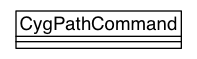
\includegraphics[width=10cm]{cdig/CygPathCommand.png}
         
 这个类只用来在windows下调用cygpath命令

    \end{XeInnerClass}
    \begin{XeInnerClass}{HardLink}
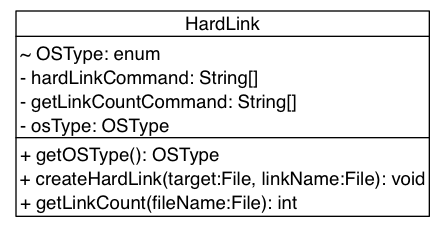
\includegraphics[width=10cm]{cdig/HardLink.png}
         
 该类抽象了硬链接
 支持unix,cygwin,windxp

        \begin{XeMethod}{\XePrivate}{OSType}{getOSType}
             
 获取系统类型

        \end{XeMethod}

        \begin{XeMethod}{\XePublic}{void}{createHardLink}
             
 创建一个硬链接

        \end{XeMethod}

        \begin{XeMethod}{\XePublic}{int}{getLinkCount}
             
 获取指定文件的链接数量

        \end{XeMethod}

    \end{XeInnerClass}
\end{XeClass}
